\hypertarget{_algorithm_8cpp}{}\section{src/\+Algorithm/\+Algorithm.cpp File Reference}
\label{_algorithm_8cpp}\index{src/\+Algorithm/\+Algorithm.\+cpp@{src/\+Algorithm/\+Algorithm.\+cpp}}
{\ttfamily \#include \char`\"{}Algorithm.\+h\char`\"{}}\newline
Include dependency graph for Algorithm.\+cpp\+:
\nopagebreak
\begin{figure}[H]
\begin{center}
\leavevmode
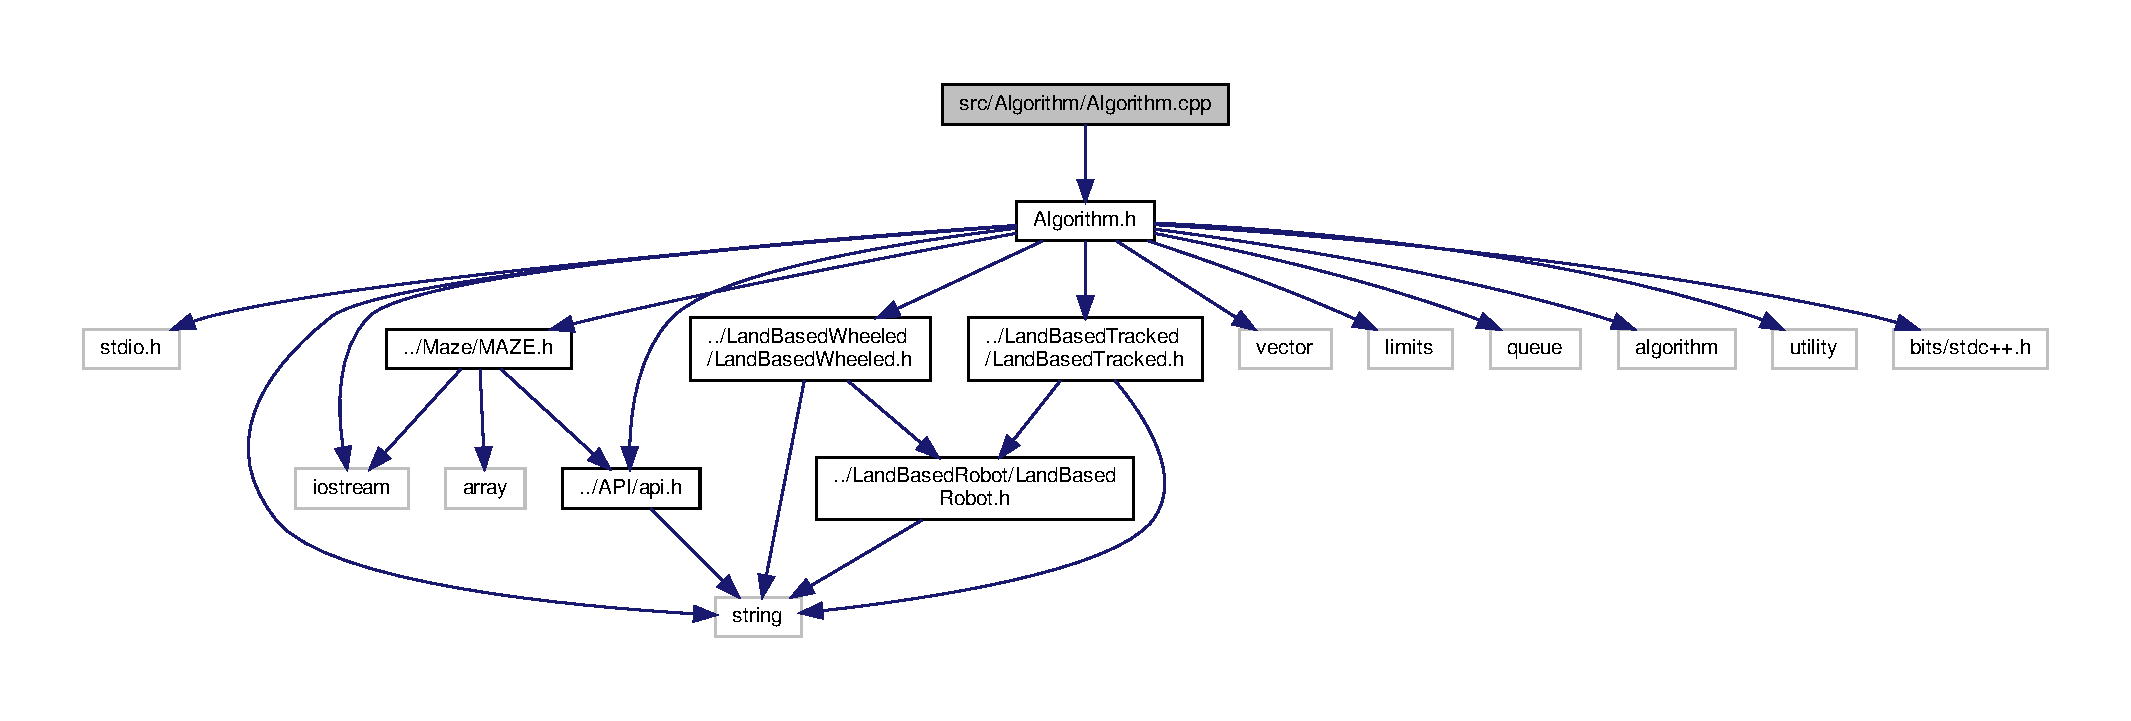
\includegraphics[width=350pt]{_algorithm_8cpp__incl}
\end{center}
\end{figure}


\subsection{Detailed Description}
\begin{DoxyAuthor}{Author}
Group9 $<$\+E\+N\+P\+M809\+Y$>$ 
\end{DoxyAuthor}
\begin{DoxyVersion}{Version}
2.\+0
\end{DoxyVersion}
\hypertarget{_m_a_z_e_8h_LICENSE}{}\subsection{L\+I\+C\+E\+N\+SE}\label{_m_a_z_e_8h_LICENSE}
This program is free software; you can redistribute it and/or modify it under the terms of the G\+NU General Public License as published by the Free Software Foundation; either version 2 of the License, or (at your option) any later version.\hypertarget{_m_a_z_e_8h_DESCRIPTION}{}\subsection{D\+E\+S\+C\+R\+I\+P\+T\+I\+ON}\label{_m_a_z_e_8h_DESCRIPTION}
This C++ program is algorithm implementation for the maze. Applied algorithm is B\+F\+S(\+Brute(\+Breadth) Force Search). All the functions are declared in the \hyperlink{_algorithm_8h}{algorithm.\+h} header file and other library have been included in header files. 